\documentclass[12pt, titlepage]{article}

\usepackage{amsmath, mathtools}
\usepackage{amsfonts}
\usepackage{amssymb}
\usepackage{graphicx}
\usepackage{colortbl}
\usepackage{xr}
\usepackage{hyperref}
\usepackage{longtable}
\usepackage{xfrac}
\usepackage{tabularx}
\usepackage{siunitx}
\usepackage{booktabs}
\usepackage{caption}
\usepackage{multirow}
\usepackage{pdflscape}
\usepackage{afterpage}
\hypersetup{
    colorlinks,
    citecolor=black,
    filecolor=black,
    linkcolor=red,
    urlcolor=blue
}
\usepackage[round]{natbib}

%% Comments

\usepackage{color}

\newif\ifcomments\commentstrue %displays comments
%\newif\ifcomments\commentsfalse %so that comments do not display

\ifcomments
\newcommand{\authornote}[3]{\textcolor{#1}{[#3 ---#2]}}
\newcommand{\todo}[1]{\textcolor{red}{[TODO: #1]}}
\else
\newcommand{\authornote}[3]{}
\newcommand{\todo}[1]{}
\fi

\newcommand{\wss}[1]{\authornote{blue}{SS}{#1}} 
\newcommand{\plt}[1]{\authornote{magenta}{TPLT}{#1}} %For explanation of the template
\newcommand{\an}[1]{\authornote{cyan}{Author}{#1}}

%% Common Parts

\newcommand{\progname}{Optimal EM Placement} % PUT YOUR PROGRAM NAME HERE
\newcommand{\authname}{Hussein Saad} % AUTHOR NAMES                  

\usepackage{hyperref}
    \hypersetup{colorlinks=true, linkcolor=blue, citecolor=blue, filecolor=blue,
                urlcolor=blue, unicode=false}
    \urlstyle{same}
                                


\begin{document}

\title{Verification and Validation Report: \progname} 
\author{\authname}
\date{\today}
	
\maketitle

\pagenumbering{roman}

\section{Revision History}

\begin{tabularx}{\textwidth}{p{3cm}p{2cm}X}
\toprule {\bf Date} & {\bf Version} & {\bf Notes}\\
\midrule
April 19, 2025 & 1.0 & Initial release\\
\bottomrule
\end{tabularx}

~\newpage

\section{Symbols, Abbreviations and Acronyms}

\renewcommand{\arraystretch}{1.2}
\begin{tabular}{l l} 
  \toprule		
  \textbf{symbol} & \textbf{description}\\
  \midrule 
  T & Test\\
  VnV & Verification and Validation\\
  SRS & Software Requirements Specification\\
  OEMP & Optimal ElectroMagnet Arrangement\\
  \bottomrule
\end{tabular}\\ \\
Units and symbols present in the \href{https://github.com/husseinsd1/optimal-em-arrangement/tree/main/docs/VnVPlan}{VnV} and \href{https://github.com/husseinsd1/optimal-em-arrangement/blob/main/docs/SRS/SRS.pdf}{SRS} apply in this document.

\newpage

\tableofcontents

\listoftables %if appropriate

\newpage

\pagenumbering{arabic}

This document provides a summary on the results of executing the test cases contained in the \href{https://github.com/husseinsd1/optimal-em-arrangement/tree/main/docs/VnVPlan}{VnV plan}. Sections \ref{fr_ev} and \ref{nfr_ev} summarize the results from test according to Sections 4.1 and 4.2 of the \href{https://github.com/husseinsd1/optimal-em-arrangement/tree/main/docs/VnVPlan}{VnV}, respectively. 

\section{Functional Requirements Evaluation} \label{fr_ev}
\subsection{Input Verification}
\begin{itemize}
  \item \textbf{Test Cases(s):} test-em-props1...6, test-inp-type-1...5, test-sys-setup-1...6
  \item \textbf{Requirements:} R1, R2
  \item \textbf{Type:} Automatic
  \item \textbf{Result Summary:} All cases passed
  \item \textbf{Logs/Re-test:} Results can be found under the \href{https://github.com/husseinsd1/optimal-em-arrangement/tree/main/cas741-oemp/cas741_oemp/tests/logs}{tests/logs} folder. To re-execute the tests, the user must run \texttt{pytest -q} in the \href{https://github.com/husseinsd1/optimal-em-arrangement/tree/main/cas741-oemp/cas741_oemp}{cas741\_oemp} directory.
\end{itemize}

\subsection{Output Verification}
\begin{itemize}
  \item \textbf{Test Cases(s):} test-output-correct-1..2
  \item \textbf{Requirements:} R6
  \item \textbf{Type:} Automatic
  \item \textbf{Result Summary:} All cases passed
  \item \textbf{Logs/Re-test:} Results can be found under the \href{https://github.com/husseinsd1/optimal-em-arrangement/tree/main/cas741-oemp/cas741_oemp/tests/logs}{tests/logs} folder. To re-execute the tests, the user must run \texttt{pytest -q} in the \href{https://github.com/husseinsd1/optimal-em-arrangement/tree/main/cas741-oemp/cas741_oemp}{cas741\_oemp} directory.
\end{itemize}

\subsection{Intermediate Value Verification}
\begin{itemize}
  \item \textbf{Test Cases(s):} test-intmed-svd-1...2
  \item \textbf{Requirements:} R3, R4, R5
  \item \textbf{Type:} Automatic
  \item \textbf{Result Summary:} All cases passed
  \item \textbf{Logs/Re-test:} Results can be found under the \href{https://github.com/husseinsd1/optimal-em-arrangement/tree/main/cas741-oemp/cas741_oemp/tests/logs}{tests/logs} folder. To re-execute the tests, the user must run \texttt{pytest -q} in the \href{https://github.com/husseinsd1/optimal-em-arrangement/tree/main/cas741-oemp/cas741_oemp}{cas741\_oemp} directory.
\end{itemize}

\section{Nonfunctional Requirements Evaluation} \label{nfr_ev}

\subsection{Accuracy}
The author was not able to generate a distribution plot, but the minimum singular values generated by OEMP were far larger than those generated by greedy/random algorithms for similar problems (unpublished work).  		


\subsection{Usability}
The author has not yet received responses from the participants of the Usability Survey. The completion of this section will be in future drafts of the document. 

\subsection{Maintainability}
The author has not yet received responses from the participants of the Usability Survey. The completion of this section will be in future drafts of the document. 

\subsection{Portability}
The author was able to able to run and pass all tests on a Windows and Linux machine. MacOS usage will be reported in future drafts.

\section{Unit Testing}
System tests verified the correctness of the Output Results Module, which in turn verified the correctness of all other modules, except the Input Parameters Module, which was verified separately (also by system tests). Thus, unit tests were deemed unnecessary. 

\section{Changes Due to Testing}
The main changes that were motivated by testing were the establishment of the Generate Poses and Magnetic Moment modules as separate ones, after they were previously local functions of other modules. Another major change was the transition from console input to a config file for entering problem related parameters.  

\section{Automated Testing}
OEMP uses \texttt{PyTest} for all testing purposes. Test cases can be found in Python files under the \href{https://github.com/husseinsd1/optimal-em-arrangement/tree/main/cas741-oemp/cas741_oemp/tests}{tests} folder. Running \texttt{pytest -q} in the \href{https://github.com/husseinsd1/optimal-em-arrangement/tree/main/cas741-oemp/cas741_oemp}{cas741\_oemp} directory will execute all tests. 

\section{Trace to Requirements}
\begin{center}
  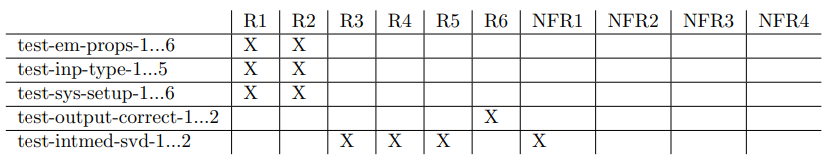
\includegraphics[scale=0.7]{TraceReq.PNG} \\
  \captionof{table}{Trace between test cases and requirements}
  \label{tracereq}
\end{center}
\newpage
\section{Trace to Modules}		
\begin{center}
  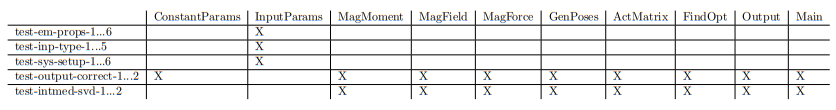
\includegraphics[scale=0.7]{TraceMod.PNG} \\
  \captionof{table}{Trace between test cases and modules}
  \label{tracemod}
\end{center}

\section{Code Coverage Metrics}
\begin{center}
  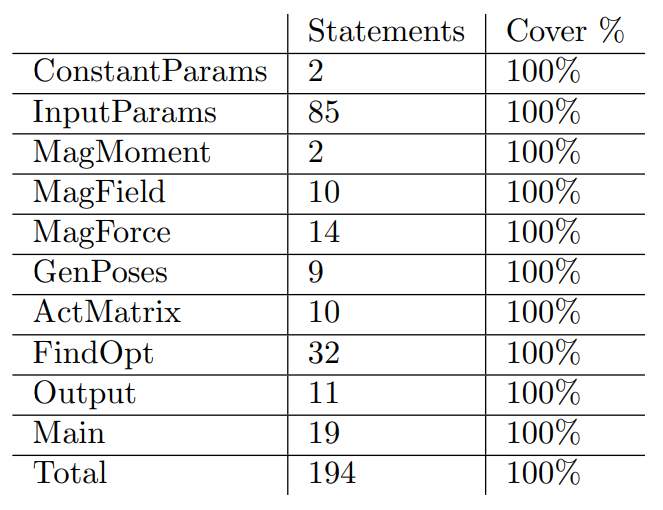
\includegraphics[scale=0.7]{Coverage.PNG} \\
  \captionof{table}{Trace between test cases and modules}
  \label{tracemod}
\end{center}


\newpage
\bibliographystyle{plainnat}
\bibliography{../../refs/References}

\end{document}